
%----------------------------------------------------------------------------------------
%	PACKAGES AND DOCUMENT CONFIGURATIONS
%----------------------------------------------------------------------------------------

\documentclass{article}

\usepackage[version=3]{mhchem} % Package for chemical equation typesetting
\usepackage{siunitx} % Provides the \SI{}{} and \si{} command for typesetting SI units
\usepackage{graphicx} % Required for the inclusion of images
\usepackage{natbib} % Required to change bibliography style to APA
\usepackage{amsmath} % Required for some math elements 
\usepackage{verbatim}
 \usepackage{float}
\usepackage{color}
\usepackage{textgreek}
\usepackage{caption}
\usepackage{subcaption}
\usepackage{fullpage}
\usepackage{listings}
\usepackage{enumitem}
\setlength\parindent{0pt} % Removes all indentation from paragraphs

\renewcommand{\labelenumi}{\alph{enumi}.} % Make numbering in the enumerate environment by letter rather than number (e.g. section 6)

%\usepackage{times} % Uncomment to use the Times New Roman font

%----------------------------------------------------------------------------------------
%	DOCUMENT INFORMATION
%----------------------------------------------------------------------------------------

\title{M3S7-Statistical Pattern Recognition  \\ Project 2} % Title

\author{Alexandre \textsc{Elkrief}\\ CID: 00732974} % Author name

\date{\today} % Date for the report

\begin{document}

\maketitle % Insert the title, author and date


% If you wish to include an abstract, uncomment the lines below
% \begin{abstract}
% Abstract text
% \end{abstract}

%----------------------------------------------------------------------------------------
%	SECTION 1
%----------------------------------------------------------------------------------------

\section{EM-Algorithm}

The density of a finite mixture distribution has the form:

$$p(\textbf x) = \sum_{i=1}^{K} \pi_{i} f_{i}(\textbf x; \boldsymbol \theta_{i})$$

where $f_i(.)$ are the $K$ component densities, and $\pi_{j}$ are mixing proportions. For fixed $K$, the EM algorithm can be used to estimate the parameters, $\boldsymbol \theta_{i}$, $\pi_{j}$, for $i = 1,...K$, from an iid sample. In this question we will restrict to all component densities being $p$-dimensional normal, with density
\\
$$f(\textbf x)=\frac{1}{(2\pi)^{\frac{p}{2}}|\boldsymbol \Sigma|^{1/2}} \exp \bigg(-\frac{1}{2}((\textbf x- \boldsymbol \mu)^{t} \boldsymbol \Sigma^{-1} (\textbf x- \boldsymbol \mu) \bigg)$$


(a) Write an R function that uses the EM algorithm to find parameters which maximise the likelihood (or minimise the negative log-likelihood) for a sample of size $n$ from $p(\textbf x)$, for a given choice of $K$. The function prototype should be \\

\textbf{em.norm(x,means,covariances,mix.prop)}\\

where \textbf x is an $n \times p$ matrix of data, \textbf{means}, \textbf{covariances}, and \textbf{mix.prop} are the initial values for the $K$ mean vectors, covariance matrices and mixing proportions. Consider including arguments, with sensible defaults, for the convergence criterion and the maximum number of iterations. \\

For the code, see appendix. I have used a convergence criterion of 0.1 between to iterations of the log-likelihood and a upper limit for the number of iterations at 100. These choices kept the computation time within reasonable bounds.\\

(b) This question will use the first two columns of the object \textbf{synth.te} in the \textbf{MASS} library: \\

\textbf{x $<-$ synth.te[,-3]}\\

For $K = 2, 3, 4, 5, 6$, use your function to compute the maximum likelihood estimates for the finite mixture of normal distributions, for these data. Select initial parameters either randomly, or by selecting from a plot of the data.

\begin{enumerate}[label=\roman*.]
\item Construct a table that reports, for each choice of $K$, the maximised likelihood, and the AIC.
\item On the basis of this table, which choice of $K$ provides the best density estimate? For this choice, construct a contour plot of the estimated density, along with the data.
\item Briefly discuss any problems you anticipate using the EM algorithm for computing a mixture model with more components, or in higher dimensions.
\end{enumerate}

i. For this question, I set the initial parameters randomly. Moreover, I chose the same AIC as in the lecture notes, namely $M=6K-1$ where K corresponds to the number of mixture components. The code outputs a matrix corresponding to the following table:\\


\begin{center}
    \begin{tabular}{ | l | l | l | p{1.5cm} |}
    \hline
    K & \ \ \ ML & \ \ AIC  \\ \hline
    2 &  &  \\ \hline
    3 &  -529.8571 & -546.8571  \\ \hline
    4 &  -486.0654 & {\color{red}-509.0654} \\ \hline
    5 &  -486.3345 &-515.3345  \\ \hline
    6 &  -485.1242 & -520.1242  \\ \hline

   
    \end{tabular}
\end{center}
\\
ii. On the basis of the above table, $K=4$ seems to be the best choice. The following plot corresponds to such a choice.

\begin{figure}[H]
\begin{center}
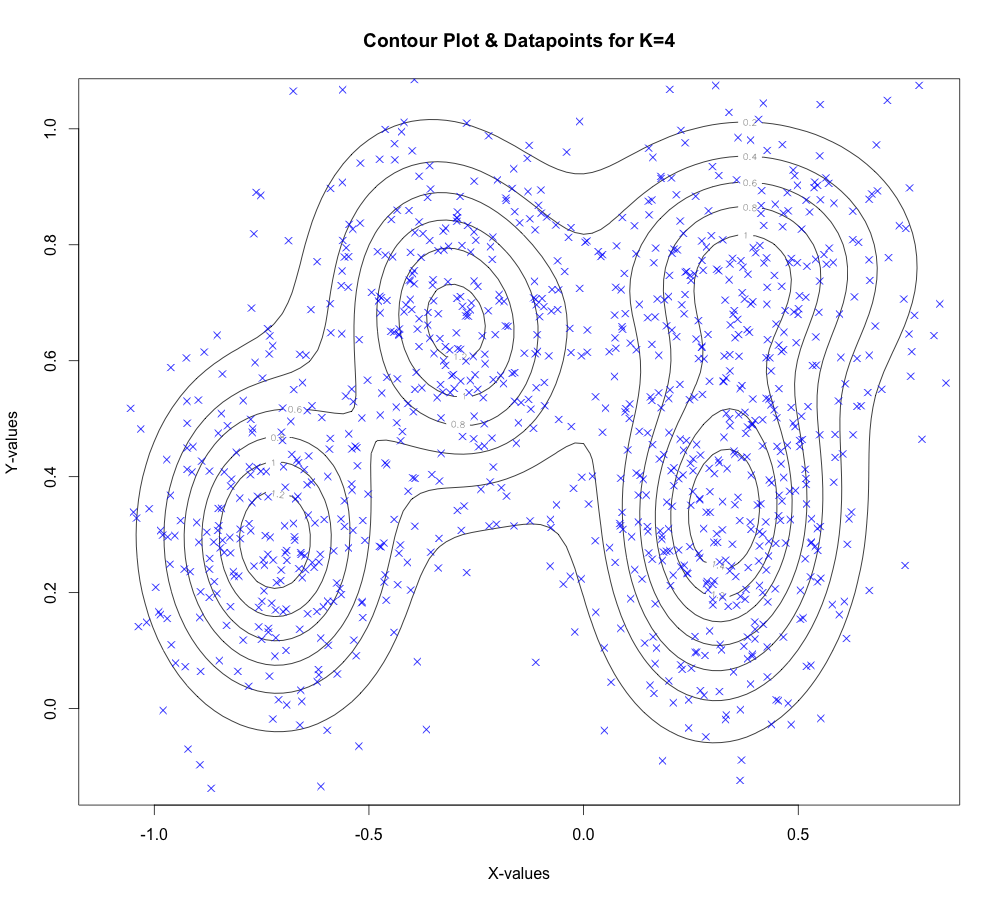
\includegraphics[width=0.65\textwidth]{Q1b} % Include the image placeholder.png
\caption{Contour plot for optimal choice of K}
\end{center}
\end{figure}

iii. The use of double for loops in my  EM-Algorithm would cause the computational time to increase exponentially when working in higher dimensions or with more mixture components.

%----------------------------------------------------------------------------------------
%	SECTION 2
%----------------------------------------------------------------------------------------

\section{Rayleigh Distribution}
Consider a two-class bivariate classification problem, with equal prior probabilities and class conditional densities given by:

$$ f(x,y|C_{i})= 4\theta_{i}^2xy\exp(-\theta_{i}(x^2+y^2)) \  \ \ \ \ x,y>0$$

and $ \theta_{i}> 0$  for $i=1,2$. Note that this joint density is the product of Rayleigh distributions.\\ 


(a) Write an R function that generates a random sample of size $n$ from class $C_{1}$ and a random sample of size $n$ for class $C_{2}$. The function should return both the feature vectors and the class indicator. A function for generating Rayleigh distributed random variables is available.\\


(b) Obtain an expression for the decision boundary for minimum error. Suppose we are interested in the situation where the decision boundary for minimum error intersects with the midpoint of the line connecting the two class mean vectors. Derive an expression for $\theta_{1}$ and $\theta_{2}$ to satisfy this situation. \\

$$ \frac{ f(x,y|C_{2})}{f(x,y|C_{1})}=\frac{p(C_{1}) }{p(C_{2} )}$$
$$ \Leftrightarrow \frac{ 4\theta_{2}^2xy\exp(-\theta_{2}(x^2+y^2)}{4\theta_{1}^2xy\exp(-\theta_{1}(x^2+y^2))}=1$$
$$\Leftrightarrow  \exp\{(x^2+y^2)(\theta_{1}-\theta_{2})\}=\frac{ \theta_{1}^2}{\theta_{2}^2}$$
$$\Leftrightarrow (x^2+y^2)(\theta_{1}-\theta_{2})=2\log(\frac{\theta_{1}}{\theta_{2}})$$
$$\Leftrightarrow T_{min}^2=x^2+y^2=2\log(\frac{\theta_{1}}{\theta_{2}})(\frac{1}{\theta_{1}-\theta_{2}})$$

As we are in 2 dimensional-space the decision boundary for minimum error is a circle on the plane. \\
 

(c) Derive an expression in terms of $\theta_{1}$ and $\theta_{2}$ for the Bayes error rate. Now, suppose $\theta_{2}=1$ and $\theta_{1}>\theta_{2}$. Use the golden ratio search algorithm developed in question 4 of project 1, to determine the value of $\theta_{1}$ that gives a Bayes error rate of 15\%. The solution occurs in the interval [3,10]. (Hint: The target function does not have to be differentiable at the minimum for the golden ratio search to work). \\

Integrating $f(x,y)$ we get: \\
$$F(x,y|C_{i})=\int_{x} \int_{y} 4\theta_{i}^2xy\exp(-\theta_{i}(x^2+y^2)) \ dx dy$$
$$\Leftrightarrow F(x,y|C_{i})=\int^{\pi/2}_{0} 2\sin(\phi)\cos(\phi) \ d\phi \int^{u}_{0} 2\theta_{i}^2r^3\exp(-\theta_{i}(r^2)) \ dr $$
$$\Leftrightarrow F(x,y|C_{i})=1-\theta_{i}u^2\exp(-\theta_{i}u^2)-\exp(-\theta_{i}u^2) $$

Now the expression for the Bayes error rate is the following: 

$$ e_{B}=p(C_{1})p(x |C_{1} \geq T)+p(C_{2})p(x|C_{2} \leq T)  $$
$$\Rightarrow e_{B}= 0.5 [(1-F_{1}(T_{min})) + F_{2}(T_{min})]$$
$$\Rightarrow e_{B}= 0.5 [(\theta_{1}T_{min}^2\exp(-\theta_{1}T_{min}^2)+\exp(-\theta_{i}T_{min}^2) + 1-\theta_{2}T_{min}^2\exp(-\theta_{2}T_{min}^2)-\exp(-\theta_{2}T_{min}^2)]$$
\\
where $T_{min}=\sqrt{2\log(\frac{\theta_{1}}{\theta_{2}})(\frac{1}{\theta_{1}-\theta_{2}})}$\\

In order to find the value of $\theta_{1}$ that gives a Bayes error rate of 15\% we use the golden ratio search algorithm to minimize the function 

$$f(\theta_{1})= |e_{B}-0.15|$$ 

This gives a value of $\theta_{1}=4.652476$\\


(d) Write down a discriminant function for each class, treating the parameter $\theta_{i}$ as unknown. \\

The code in the appendix uses the following discriminant function:
$$g_{i}(\textbf{x})=\log(p(C_{i})+\log(p(\textbf{x}|C_{i}))$$ 

(e) Let $\theta_{1}=4$ and $\theta_{2}=2$. Construct a plot of the unconditional density 
$$f(x,y)=p(C_{1})f(x,y|C_{1})+p(C_{2})f(x,y|C_{2})$$
 for the specified parameter values. Obtain a sample of 50 observations from each class. Add these data and the Bayes optimal decision boundary to the plot. \\

\begin{figure}[H]
\begin{center}
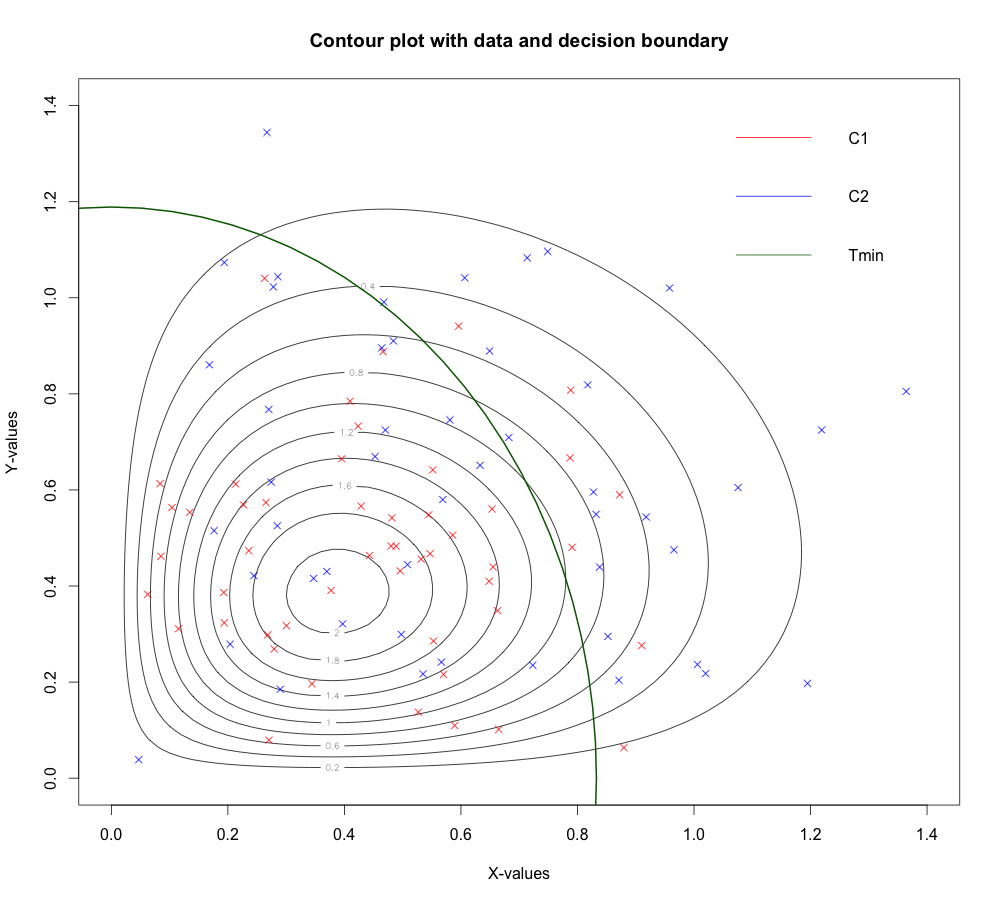
\includegraphics[width=0.65\textwidth]{Q2e} % Include the image placeholder.png
\caption{Unconditional Density and Decision Boundary}
\end{center}
\end{figure}

(f) Derive the maximum likelihood estimators for the parameters of each class, given a sample of size $n$ from each class. \\

$$l(\theta_{j})=\sum_{i=1}^{n} \log(f(x_{i},y_{i}|\theta_{j})$$
$$\Leftrightarrow l(\theta_{j})=\sum_{i=1}^{n} \log(4\theta_{j}^2x_{i}y_{i}\exp(-\theta_{j}(x_{i}^2+y_{i}^2)))$$
$$\Leftrightarrow  l(\theta_{j})=\sum_{i=1}^{n} -\theta_{j}(x_{i}^2+y_{i}^2) + 2\log(2\theta_{j})+\log(x_{i}y_{i})$$
$$\Leftrightarrow  l(\theta_{j})= -\theta_{j} \sum_{i=1}^{n}(x_{i}^2+y_{i}^2) +\sum_{i=1}^{n} \log(x_{i}y_{i})+ 2n\log(2\theta_{j})$$

$$\Rightarrow \frac{\partial l}{\partial \theta_{j}}=0$$
$$\Rightarrow -\sum_{i=1}^{n}(x_{i}^2+y_{i}^2) + \frac{2n}{2\theta_{j}}=0$$
$$\Rightarrow  \widehat{\theta_{j}}=\frac{2n}{\sum_{i=1}^{n}(x_{i}^2+y_{i}^2)}$$
$$ $$


(g) Write two R functions, the first for computing the maximum likelihood estimates in (f) from a set of data generated by the function in (a), and the second for evaluating the discriminant function for each class, using the maximum likelihood estimates (the estimative discriminant function). Compute the discriminant scores for the data generated in (e) and estimate the error rate of this classifier on this training data. \\

The discriminant scores are computed within the discriminant function which allocates each points to one of the 2 classes.\\
The error rate of this classifier ranges between  25\%  and 37\% depending on the set of points generated.\\
(see code in appendix)\\


(h) Obtain a training sample of size $n = 200$ and a test sample of size $n = 10000$, using the parameter values in part (e). Retain these training and test samples for use in Questions 3 and 4. Using these data sets, compute the training and test set error rates for
\begin{enumerate}[label=\roman*.]
\item the estimative version of the true model, using the functions in part (g),
\item Linear discriminant analysis,
\item Quadratic discriminant analysis.
\end{enumerate}
Provide a table of these error rates for the different models. Comment on the results.\\


The table of error rates is the following:

\begin{center}
    \begin{tabular}{ | l | l | l | p{1.5cm} |}
    \hline
    Dataset & ML model& LDA & QDA \\ \hline
    Training & 33.5\% & 34.5\% & 33.5\% \\ \hline
    Testing & 32\% & 32.8\% & 32.4\% \\ \hline
   
    \end{tabular}
\end{center}




%----------------------------------------------------------------------------------------
%	SECTION 3
%----------------------------------------------------------------------------------------

\section{Kernel Density Estimation }

This question is concerned with product kernel classifiers, based on a density estimate of the form:
$$ \hat p(\boldsymbol x^{*})= \frac{1}{n}\frac{1}{h_{1}h_{2}...h_{d}} \sum_{i=1}^n \prod_{j=1}^n K\bigg( \frac{[\boldsymbol x^{*} - \boldsymbol x_{i}]_{j}}{h_{j}} \bigg)

where $d$ is the dimension of the feature vector, $K()$ is a kernel function, $n$ is the number of observations in the sample, and $h_{j} j = 1,2,...,d$, are bandwidth parameters. Restrict attention to the normal kernel:

$$K(z) = \frac{1}{\sqrt{2\pi}}\exp{\bigg(\frac{-z^2}{2}\bigg)} $$


(a) Write a function with prototype \textbf{kde(x.star,data,bw)} that will perform a kernel density estimate for a single $d$-dimensional feature vector  \textbf{x.star}, using an $n \times d$ data set data and $d$ bandwidth parameters contained in a vector  \textbf{bw}.\\

(b) A classifier proceeds by evaluating a probability density estimate for each class, given bandwidth parameters, and combines these with information about prior probabilities, to obtain estimated posterior probabilities of class membership. In this question, we will use the same bandwidth parameters for both classes.\\
Using the data you generated in Question 2 part (h) (so $d$ = 2), perform a 2-fold cross-validation for bandwidth selection in the following manner (you may take the class priors as $P(C_{1}) = P (C_{2}) = 0.5$):

\begin{enumerate}[label=\roman*.]
\item Randomly split the training data generated in Question 2 (h) into two blocks of 100 samples each, $D_1$ and $D_2$, say.
\item Construct a $20\times 20$ grid of values for $H$ = ($h1, h2$) defined on $[0.05, 1] \times [0.05, 1]$, where $h_j$ is the bandwidth parameter for variable $j$. For each selection of $H$:
\begin{itemize}
\item Classify each observation in $D_2$, using $D_1$ as the training set. Compute and retain the error rate.
\item Classify each observation in $D_1$, using $D_2$ as the training set. Compute and retain the error rate.
\item Combine these two error rates to give an average error rate for this selection of $H$.
\end{itemize}
\end{enumerate}



(c) What is the minimum error rate found in part (b), and what are the associated bandwidths $h_1$ and $h_2$?\\ 

The minimum error rate is --- , corresponding to $(h_1,h_2)=( -,-)$\\

(d) For this  $h_1$ and $h_2$ use all your training data and calculate the error rate on the 10000 test sample generated in Question 2 (h). \\

The error rate we obtain using the the best choice of $(h_1,h_2)$ is ---.






%----------------------------------------------------------------------------------------
%	SECTION 4
%----------------------------------------------------------------------------------------

\section{Distance-weighted K-NN}

In an early attempt to combine the features of kernel methods and $k$-nearest neighbour methods, Dudani $(1976)^2$ proposed a $distance \ weighted$ version of the $k$-nearest neighbour classifier. In this version, weights are assigned to the $k$-nearest neighbours, with closer neighbours being weighted more heavily. A feature vector \textbf{x} is then assigned to the class for which the weights of the representatives among the $k$ neighbours sum to the greatest value.\\
One implementation of this strategy is as follows. For a specific feature vector, \textbf{x}, let the number of neighbours of class $i$ among the $k$-nearest neighbours be $k_{i}, i = 1,2,...,K$, where $K$ is the number of classes. Note that $\sum_{i=1}^{K} k_{i} = k$. Let the Euclidean distance of \textbf{x} from each of these class $i$ neighbours be $d_{i}^{j}$, for $j = 1,2,...,k_{i}$. The $weight$ associated with class $i$ is
$$ w_{i}=\sum_{j=1}^{k_{i}} f(d_{i}^{j}) \ \ \ i= 1,2,...,K$$

A popular choice for the weighting function$f$ (in the nonparametric smoothing literature) is the $tricube$ function

$$f(x)=(1-|x|^3)^3$$

for $|x| \leq 1$, and 0 otherwise. This requires that we re-scale the distances, $d_{i}^{j}$ , such that the largest, for all $i$ and $j$, is 1. The allocation rule is then: allocate to class $i$ if $w_{i} >w_{j}$ for all $j\not=i$.

(a) Write an R function that implements the procedure described above. The function prototype should be of the form\\ \\
\textbf{knn.dist(train,test,class,k)} \\

where \textbf{train} is a matrix of training data (the rows are feature vectors), \textbf{class} is the associated vector of class indicators, \textbf{test} is a matrix of test data, and \textbf{k} is the number of neighbours.\\

(b) Using the training data obtained in Question 2 (h), perform a 2- fold cross-validation to select $k$ from $k = 3, 7, 11, 15, 19, 23, 27, 31, 35$ or 39 for your distance weighted $k$-nearest neighbour classifier.\\

(c) For your selection of $k$ use all your training data and calculate the error rate on the 10000 test sample from Question 2 (h).\\



(d) You have now tried various methods on these data. Discuss the method you prefer for this problem and issues that motivate your preference. \\

Considering methods from Q2, Q3 and Q4, the Kernel density estimation method from question 2 is the most computationally expensive. Working in higher dimensions and with a bigger range for each bandwidth parameter increases the computational time significantly as the number of combinations of $h_1,h_2,...,h_d$ increased exponentially. Moreover, this method doesn't produce significantly better error rates, at least in the case of our data. 

The other methods give similar error rates and are similarly quick to run (although finding the optimal choice of K in Q4 isn't instantaneous). I would therefore use a combination of these 4 methods (ML, LDA, QDA and Distance-weighted K-NN) depending on the set of data that I need to test.


\newpage
\section{Appendix}
\lstset{
basicstyle=\small\ttfamily,
columns=flexible,
breaklines=true
}
\begin{lstlisting}



\end{lstlisting}
%----------------------------------------------------------------------------------------
%	BIBLIOGRAPHY
%----------------------------------------------------------------------------------------

%\bibliographystyle{apalike}

%\bibliography{sample}

%----------------------------------------------------------------------------------------


\end{document}